
\section{Calibração Intrínseca}

Para realização da calibração intrínseca da câmera, foram tomadas duas capturas de um objeto de calibração, sendo essa, uma caixa conhecida com 275 mm de altura, 87 mm de largura e 150 mm de profundidade. A \autoref{fig:i7_L} apresenta a vista esquerda da caixa, enquanto na \autoref{fig:i7_R} foi capturada a vista direita do objeto.

\begin{figure}[H]
	\centering
	\begin{subfigure}[H]{0.49\textwidth}
		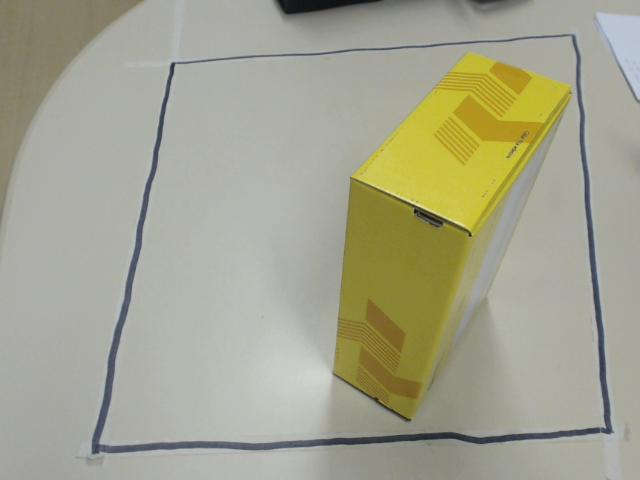
\includegraphics[width = \textwidth]{../../data/i7_L.jpg}
		\caption{Vista esquerda.}
		\label{fig:i7_L}
	\end{subfigure}
	\begin{subfigure}[H]{0.49\textwidth}
		\centering
		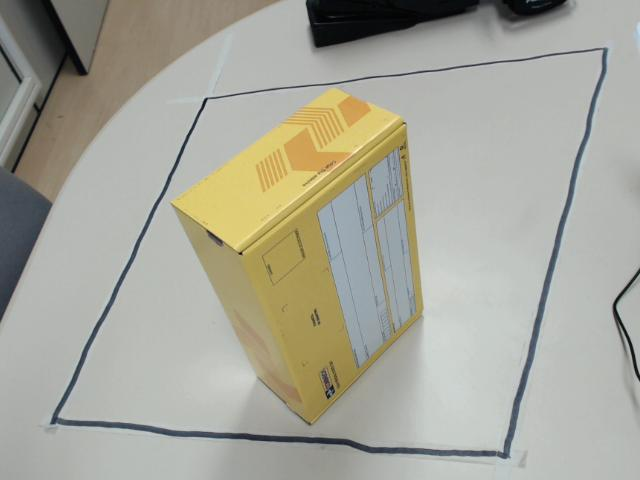
\includegraphics[width = \textwidth]{../../data/i7_R.jpg}
		\caption{Vista direita.}
		\label{fig:i7_R}
	\end{subfigure}
	\caption{Imagens de calibração.}
\end{figure}

\subsection{Obtenção de pontos}

A definição dos pontos do sólido de calibração que serão utilizados para a calibração é crucial, tendo sido realizado de forma manual por meio do \textit{software} de edição de imagens Adobe Photoshop. Os pontos são enumerados para corresponder ao vetor de pontos conhecidos utilizados na função de calibração, sendo o sistema global de coordenadas tendo origem no ponto $\mathit{1}$ e os eixos definidos nas direções:

\begin{align}
	\text{Eixo } z \equiv \overrightarrow{\mathit{1} \to \mathit{6}} \\
	\text{Eixo } x \equiv \overrightarrow{\mathit{1} \to \mathit{2}} \\
	\text{Eixo } y \equiv \overrightarrow{\mathit{1} \to \mathit{7}}
\end{align}

O ponto oculto foi estimado por meio da projeção das arestas ocultas do sólido, por meio do paralelismo com as arestas visíveis, onde o ponto de interseção foi aproximado como o oitavo vértice do paralelepípedo.

\begin{figure}[H]
	\centering
	\begin{subfigure}[H]{0.49\textwidth}
		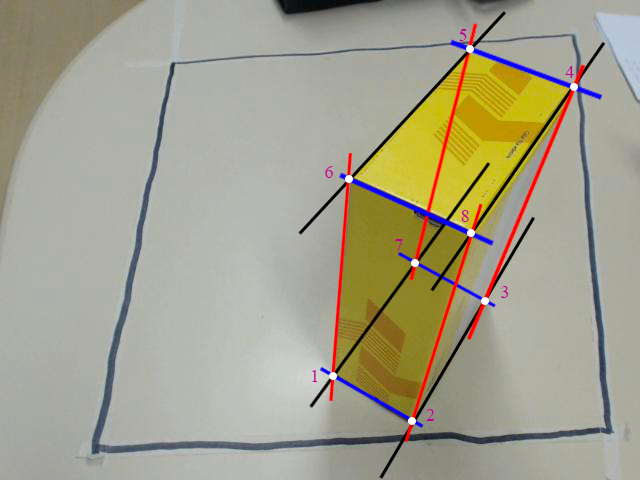
\includegraphics[width = \textwidth]{../../data/i7_L_axis.png}
		\caption{Vista esquerda.}
		\label{fig:i7_L_axis}
	\end{subfigure}
	\begin{subfigure}[H]{0.49\textwidth}
		\centering
		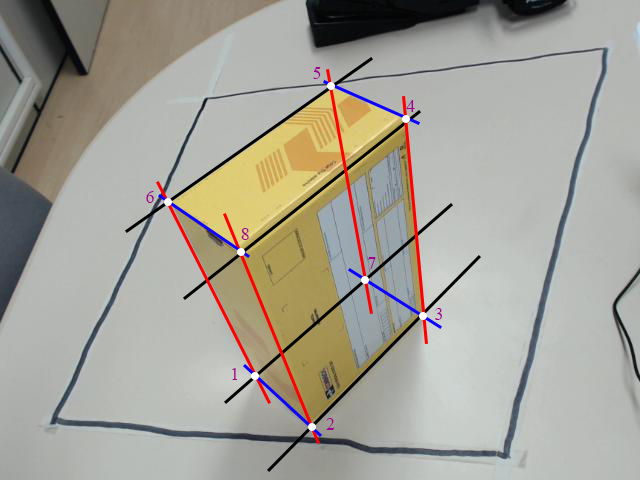
\includegraphics[width = \textwidth]{../../data/i7_R_axis.png}
		\caption{Vista direita.}
		\label{fig:i7_R_axis}
	\end{subfigure}
	\caption{Imagens de calibração com pontos conhecidos do mundo destacados.}
\end{figure}

Os pontos foram amostrados manualmente da imagem com os eixos, utilizando a função \texttt{getpts} do \textsc{Matlab}, resultando em dois vetores, com as coordenadas $x$ e $y$ de cada ponto. Dado as coordenadas, os mesmos foram utilizados para montar a matriz de pontos de calibração, com o mesmo padrão mostrado em \eqref{eq:mpoints}, sendo \texttt{ceil()} a função de truncamento para obtenção da coordenada de imagem do ponto, sendo obtida uma matriz de pontos para cada imagem.

\begin{equation}\label{eq:mpoints}
	\+p = \begin{bmatrix}
		\texttt{ceil(}\vec{x}\texttt{)}_{[1 \times 8]} \\
		\texttt{ceil(}\vec{y}\texttt{)}_{[1 \times 8]} \\
		\mathbf{1}
	\end{bmatrix}_{[3 \times 8]}
\end{equation}

Com a aplicação da função de calibração intrínseca \texttt{RTAa()}, obtém-se a matriz de parâmetros intrínsecos aproximada ($\mathbf{\hat{A}}$), a matriz de rotação aproximada ($\mathbf{\hat{R}}$) e o vetor de translação aproximado ($\mathbf{\hat{t}}$), sendo os dois últimos em relação à câmera e o sistema de coordenadas do mundo, ou seja, serão diferentes para cada uma das imagens.

Para a vista esquerda (\autoref{fig:i7_L_axis}), foram obtidas as seguintes matrizes:

\begin{gather}\label{eq:ve}
\hat{\+A}_L = \begin{bmatrix}
	582.1562 & 0        & 853.3215 \\
	0        & 680.1808 & 561.4679 \\
	0        & 0        & 1  
\end{bmatrix}; \\ \ \hat{\+R}_L = \begin{bmatrix}
	0.7061  &  0.1509  &  0.6919 \\
	0.3502  & -0.9236  & -0.1559 \\
	0.6155  &  0.3524  & -0.7050
\end{bmatrix}; \ \hat{\+t}_L = \begin{bmatrix}
	-0.0657 \\
	 0.2558 \\
	-0.7038
\end{bmatrix};  \label{eq:rtL}
\end{gather}

Para a vista direita (\autoref{fig:i7_R_axis}), foram obtidas as seguintes matrizes:

\begin{gather}\label{eq:vd}
	\hat{\+A}_R = \begin{bmatrix}
	623.9344 & 0        & 322.8278 \\
	0        & 585.1104 & 182.6302 \\
	0        & 0        & 1.0000
	\end{bmatrix}; \\ \ \hat{\+R}_R = \begin{bmatrix}
	0.6818  &  0.7061 &  -0.1912 \\
	0.4016  & -0.5797 &  -0.7090 \\
	-0.6114 &  0.4066 &  -0.6788
	\end{bmatrix}; \ \hat{\+t}_R = \begin{bmatrix}
	 0.3196 \\
	-0.0838 \\
	 0.5338
	\end{bmatrix}; \label{eq:rtR}
\end{gather}

Por fim, para uma melhor realização da matriz de parâmetros intrínsecos aproximada, tira-se a média das duas aproximações obtidas, tendo então:

\begin{equation}\label{eq:amed}
	\hat{\+A} = \begin{bmatrix}
		603.0453 & 0        & 588.0747 \\
		0        & 632.6456 & 372.0490 \\
		0        & 0        & 1.0000
		
	\end{bmatrix}
\end{equation}



\section{Transformação entre às câmeras}

A matriz de rotação e o vetor de translação entre a câmera e o sistema de coordenadas do mundo podem ser representadas na forma de transformações homogêneas, que compactam a informação de rotação e translação, sendo construída com base em \eqref{eq:th}.

\begin{equation}
	\+T = \begin{bmatrix}
	&	\+R_{[3\times 3]} & & \+{t}_{[3\times 1]} \\
		0 & 0 & 0 & 1
	\end{bmatrix}_{[4\times 4]}
	\label{eq:th}
\end{equation}

Para a transformação entre dois \textit{frames} $\{2\}$ e $\{1\}$ quaisquer, tem-se \eqref{eq:th21}.

\begin{equation}
\+T_{2/1} = \begin{bmatrix}
	& \+R_{2/1} & & \+v{t}_{2/1} \\
	0 & 0 & 0 & 1
\end{bmatrix}
\label{eq:th21}
\end{equation}

De acordo com a propriedade algébrica das transformações homogêneas, a transformação do \textit{frame} $\{0\}$ para o $\{2\}$ pode ser decomposta no produto da transformação do \textit{frame} $\{0\}$ para o $\{1\}$, e do   \textit{frame} $\{1\}$ para o $\{2\}$.

\begin{equation}
	\+T_{0/2} = \+T_{2/1} \+T_{1/0} \therefore \+T_{2/1} = \+T_{0/2} \+T_{1/0} = \+T_{0/2} \+T^{-1}_{0/1}
\end{equation}

Dessa forma, uma vez que se conhece a transformação da câmera na vista esquerda para o sistema do mundo, e a transformação da câmera na vista direita para o sistema do mundo, a tranformação entre as duas câmeras pode ser encontrada da forma \eqref{eq:tfLR}.

\begin{equation}
	\+T_{R/L} = \+T_{R/0}\+T_{0/L} =  \+T_{R/0}\+T_{L/0}^{-1}
	\label{eq:tfLR}
\end{equation}

Com base em \eqref{eq:rtL}, pode-se escrever a transformação homogênea da câmera L para o sistema de coordenadas do mundo como \eqref{eq:TL}

\begin{equation}\label{eq:TL}
	\+T_{L/0} = \begin{bmatrix}
		& \hat{\+R}_L & & \hat{\+t}_L\\
		0 & 0 & 0 & 1
	\end{bmatrix} = \begin{bmatrix}
	0.7061  &  0.1509  &  0.6919 & -0.0657 \\
	0.3502  & -0.9236  & -0.1559 & 0.2558  \\
	0.6155  &  0.3524  & -0.705  & -0.7038 \\
	0       &  0      &   0      & 1
\end{bmatrix}
\end{equation}  

E por meio da \eqref{eq:rtR}, pode-se escrever a transformação homogênea da câmera R para o sistema de coordenadas do mundo como \eqref{eq:TR}

\begin{equation}\label{eq:TR}
 	\+T_{R/0} = \begin{bmatrix}
 		& \hat{\+R}_R & & \hat{\+t}_R\\
 		0 & 0 & 0 & 1
 	\end{bmatrix} = \begin{bmatrix}
 	0.6818  &  0.7061 &  -0.1912 & 0.3196  \\
 	0.4016  & -0.5797 &  -0.7090 & -0.0838 \\
 	-0.6114 &  0.4066 &  -0.6788 & 0.5338  \\
 	0       &  0      &   0      & 1
 \end{bmatrix}
\end{equation} 


Com isso, de acordo com \eqref{eq:tfLR}, têm-se que, a transformação do referencial da câmera da esquerda para a câmera da direta é expressa por \eqref{eq:tfL2R} e a transformação da câmera da direta para a câmera da esquerda é dada por \eqref{eq:tfR2L}.

\begin{equation}\label{eq:tfL2R}
	\+T_{L/R} = \begin{bmatrix}
		0.2457  &  0.5458  & -0.8011 &   0.9148 \\
		-0.4834 &  0.7853  &  0.3867 &   0.8080 \\
		0.8402  &  0.2922  &  0.4568 &  -0.5530 \\
		0       &  0       &  0      &   1
	\end{bmatrix}
\end{equation}

\begin{equation}\label{eq:tfR2L}
	\+T_{R/L} = \begin{bmatrix}
		0.2457  &  -0.4834 &  0.8402  &  0.6304 \\
		0.5458  &  0.7853  &  0.2922  & -0.9722 \\
		-0.8011 &  0.3867  &  0.4568  &  0.6730 \\
		0       &  0       &  0       &  1
	\end{bmatrix}
\end{equation}
